
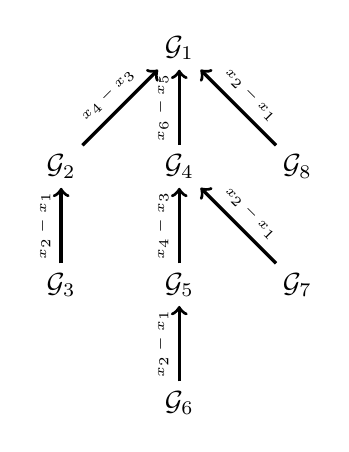
\begin{tikzpicture}[scale = 0.5]

\node (A) at (0,0) {$\mathcal{G}_{1}$};

\node (C) at (-3,-3) {$\mathcal{G}_{2}$};
\node (D) at (0,-3) {$\mathcal{G}_{4}$};
\node (B) at (3,-3) {$\mathcal{G}_{8}$};

\node (E) at (3,-6) {$\mathcal{G}_{7}$};
\node (F) at (-3,-6) {$\mathcal{G}_{3}$};
\node (G) at (0,-6) {$\mathcal{G}_{5}$};

\node (H) at (0,-9) {$\mathcal{G}_{6}$};


\draw[->, very thick] (D) to node[midway, above, sloped]   {\tiny{$x_{6}-x_{5}$}} (A);
\draw[->, very thick] (C) to node[midway, above, sloped]   {\tiny{$x_{4}-x_{3}$}} (A);
\draw[->, very thick] (B) to node[midway, above, sloped]   {\tiny{$x_{2}-x_{1}$}} (A);

\draw[->, very thick] (E) to node[midway, above, sloped]   {\tiny{$x_{2}-x_{1}$}} (D);
\draw[->, very thick] (F) to node[midway, above, sloped]   {\tiny{$x_{2}-x_{1}$}} (C);
\draw[->, very thick] (G) to node[midway, above, sloped]   {\tiny{$x_{4}-x_{3}$}} (D);

\draw[->, very thick] (H) to node[midway, above, sloped]   {\tiny{$x_{2}-x_{1}$}} (G);


\end{tikzpicture}
